\section{Further absorption models}
\label{m:app:moc}

The models considered so far describe the population inside a single compartment.
Once several compartments share a medium, a further question arises: what becomes
of the contents of the first compartment to rupture? The shared medium acquires,
at a stroke, a potentially large cohort of particles available for subsequent
absorption by the compartments that remain. This appendix treats the case in
which a cohort of particles enters a single compartment, by the method of
\cref{m:sec:moc}: the absorption-only model, which is simpler than the
worked example of \cref{m:sec:mocabsdeath} and serves as a check case, and the
absorption--birth--death model, which is harder than it and whose closed form,
\cref{m:prop:Gabd}, is a result of this thesis.

\subsection{Absorption only}
\label{m:sec:absonly}

The simplest absorption process has a single compartment that takes in
particles, with no subsequent dynamics: no birth and no death within the
compartment.

Let $X_t$ and $Y_t$ count the particles inside and outside the compartment
respectively; the same labelling is used for every version of the
single-compartment model below. Events are stochastic with exponentially
distributed inter-event times, which by \cref{m:sec:exp} follows from the
assumption that event rates do not depend on time, so that
$\{(X_t,Y_t):t\ge0\}$ is a continuous-time Markov chain in the sense of
\cref{m:sec:generator}.

With only absorption to consider, the model is specified by the transition
probabilities over an infinitesimal interval $\Delta t$,
\begin{align*}
\pr{\Delta X = 1,\ \Delta Y = -1 \mid Y_t = j} &= j\alpha\,\Delta t, &&\text{(absorption)}\\
\pr{\Delta X = 0,\ \Delta Y = 0 \mid Y_t = j} &= 1-j\alpha\,\Delta t, &&\text{(no event)}
\end{align*}
where $\Delta X = X_{t+\Delta t}-X_t$ and similarly for $Y$, and terms of
$o(\Delta t)$ are suppressed throughout. The factor $j$ records that each
exterior particle is independently subject to the same probability
$\alpha\Delta t$ of being taken up. The initial condition is $X_0=0$, $Y_0=N$:
a starter population of $N$ particles occupying the exterior medium.

Writing $p_{i,j}(t) = \pr{X_t=i,\ Y_t=j}$, the forward Kolmogorov equations
are
\begin{equation}
\label{m:eq:FK1}
\ddt{p_{i,j}} = \alpha(j+1)p_{i-1,j+1} - \alpha j\,p_{i,j} .
\end{equation}
With the bivariate generating function
\begin{equation}
\label{m:eq:pgfbiv}
G(x,y,t) = \sum_i\sum_j p_{i,j}(t)\,x^iy^j = \ex{x^{X_t}y^{Y_t}},
\end{equation}
\cref{m:eq:FK1} converts into a partial differential equation by the procedure
of \cref{m:sec:pgf}. Multiply each equation by $x^iy^j$ and sum over $i$ and
$j$; the sums are finite, because $p_{i,j}(t)=0$ whenever $i+j\neq N$,
particles in this model being neither created nor destroyed. Shifting indices
in the first term sends $\alpha(j+1)p_{i-1,j+1}x^iy^j$ to
$\alpha x\,\partial_yG$, and the second term is $-\alpha y\,\partial_yG$, so
that
\begin{equation}
\label{m:eq:PDE1}
\pddt{G} = \alpha(x-y)\pdd{G}{y},
\qquad G(x,y,0) = y^N .
\end{equation}
The method of characteristics of \cref{m:sec:mocrecipe} applies to
\cref{m:eq:PDE1} as it does to \cref{m:eq:PDE2}, but the solution can be
obtained more quickly by exploiting the independence that this model retains,
and that route also provides a check on the machinery.

\subsubsection*{Exploiting independence}

The function $G$ above was specific to $X_0=0$, $Y_0=N$. Define more generally
\begin{equation*}
G_n(x,y,t) = \sum_i\sum_j\pr{X_t=i,\ Y_t=j \mid X_0=0,\ Y_0=n}\,x^iy^j .
\end{equation*}
In a process of pure absorption the $n$ particles are taken up one by one, and
the behaviour of any one of them does not depend on the movements of its
neighbours. That independence lets $X_t$ and $Y_t$ decompose into sums of $n$
single-particle variables,
\begin{equation*}
X_t = \sum_{k=1}^{n}X_t^{(k)},
\qquad
Y_t = \sum_{k=1}^{n}Y_t^{(k)},
\end{equation*}
from which
\begin{equation}
\label{m:eq:indRelPGF}
G_n(x,y,t) = \bigl(G_1(x,y,t)\bigr)^n ,
\end{equation}
since
\begin{equation*}
G_n(x,y,t)
= \ex{\prod_{k=1}^{n}x^{X_t^{(k)}}\prod_{k=1}^{n}y^{Y_t^{(k)}}}
= \prod_{k=1}^{n}\ex{x^{X_t^{(k)}}y^{Y_t^{(k)}}}
= \bigl(G_1(x,y,t)\bigr)^n .
\end{equation*}

Now consider a single initial particle, $X_0=0$, $Y_0=1$. It is eventually
absorbed, and that is the final state of the system: no other states are
reachable, so $p_{i,j}(t)=0$ whenever $i+j\neq1$. The forward equations reduce
to
\begin{equation*}
\ddt{p_{0,1}} = -\alpha p_{0,1},
\qquad
\ddt{p_{1,0}} = \alpha p_{0,1},
\end{equation*}
giving $p_{0,1}(t) = \ee^{-\alpha t}$ and $p_{1,0}(t) = 1-\ee^{-\alpha t}$
(\cref{m:fig:abs1}). These being the only two non-zero state probabilities of
the single-particle system,
\begin{equation*}
G_1(x,y,t) = p_{1,0}(t)\,x + p_{0,1}(t)\,y
= \lrb{1-\ee^{-\alpha t}}x + \ee^{-\alpha t}y ,
\end{equation*}
and \cref{m:eq:indRelPGF} gives the generating function for any initial
census,
\begin{equation}
\label{m:eq:Gabsonly}
G_n(x,y,t) = \Bigl(\lrb{1-\ee^{-\alpha t}}x + \ee^{-\alpha t}y\Bigr)^n .
\end{equation}
This satisfies \cref{m:eq:PDE1} together with the initial condition
$G_n(x,y,0)=y^n$. The form is recognisable:
$X_t\sim\text{Binomial}(n,1-\ee^{-\alpha t})$, as it must be, since the $n$
particles are absorbed independently and each has been taken up by time $t$
with probability $1-\ee^{-\alpha t}$.

\begin{figure}[H]
\centering
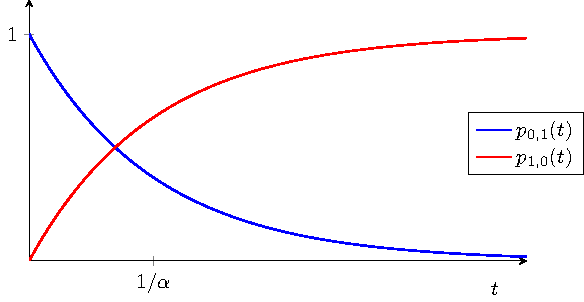
\includegraphics[width=0.62\textwidth]{figures/abs1.pdf}
\caption{State probabilities for the single-particle absorption-only model. The
particle begins outside the compartment ($p_{0,1}$, decaying exponentially at
rate $\alpha$) and ends inside it ($p_{1,0}$). There is nowhere else for it to
go, so the two curves sum to one at every time.}
\label{m:fig:abs1}
\end{figure}

\subsection{Absorption--birth--death}
\label{m:sec:absbirthdeath}

Introducing replication for particles inside the compartment, the independence
property is still present but no longer serves as a shortcut: from a single
initial particle, birth events make infinitely many states reachable, so
$G_1(x,y,t)$ is an infinite sum and there is nothing to be gained by
factorising. The partial differential equation must therefore be solved
directly, and by now that can be done.\footnote{I am grateful to Benjamin Sharp
for the advice on applying the method of characteristics to three-variate
problems that unlocked this calculation.}

With $X_t$ and $Y_t$ as before, birth at per-capita rate $\lambda$ is added to
the transition probabilities:
\begin{align*}
\pr{\Delta X = 1,\ \Delta Y = -1 \mid Y_t=j} &= j\alpha\,\Delta t, &&\text{(absorption)}\\
\pr{\Delta X = 1,\ \Delta Y = 0 \mid X_t=i} &= i\lambda\,\Delta t, &&\text{(birth)}\\
\pr{\Delta X = -1,\ \Delta Y = 0 \mid X_t=i} &= i\mu\,\Delta t, &&\text{(death)}\\
\pr{\Delta X = 0,\ \Delta Y = 0 \mid X_t=i,\ Y_t=j} &= 1-(j\alpha+i\mu+i\lambda)\Delta t, &&\text{(no event)}
\end{align*}
with forward Kolmogorov equation
\begin{equation}
\label{m:eq:FK3}
\ddt{p_{i,j}} = \alpha(j+1)p_{i-1,j+1} + \mu(i+1)p_{i+1,j} + \lambda(i-1)p_{i-1,j}
- (\alpha j+\mu i+\lambda i)p_{i,j} .
\end{equation}
The same reasoning as before gives the generating-function equation
\begin{equation}
\label{m:eq:PDE3}
\pddt{G} = \bigl(\mu-(\mu+\lambda)x+\lambda x^2\bigr)\pdd{G}{x} + \alpha(x-y)\pdd{G}{y},
\qquad G(x,y,0)=y^N ,
\end{equation}
whose $x$-coefficient is exactly the quadratic met in \cref{m:eq:bdpde} for the
linear birth--death process. Reparametrising $(x,y,t)\to(\sigma,\eta,\tau)$ as
in the worked example of \cref{m:sec:mocabsdeath} gives the characteristic
system
\begin{align}
\dda{G}{\tau} &= 0, \label{m:eq:ch21}\\
\dda{t}{\tau} &= -1, \label{m:eq:ch22}\\
\dda{x}{\tau} &= \mu-(\mu+\lambda)x+\lambda x^2, \label{m:eq:ch23}\\
\dda{y}{\tau} &= \alpha(x-y), \label{m:eq:ch24}
\end{align}
with the same initial conditions \cref{m:eq:ICpar}.

\paragraph{The equations for $G$ and $t$, \eqref{m:eq:ch21}--\eqref{m:eq:ch22}.}
As before,
\begin{equation}
\label{m:eq:GetaN2}
G(\sigma,\eta,\tau) = \eta^N,
\qquad
t = -\tau .
\end{equation}

\paragraph{The equation for $x$, \eqref{m:eq:ch23}.}
This is a Riccati equation of the same shape as the one governing the survival
probability in \cref{m:app:critical}. Its right-hand side factorises, and the
roots are elementary rather than the surd expression that mechanical use of the
quadratic formula suggests:
\begin{equation}
\label{m:eq:xpm}
\mu-(\mu+\lambda)x+\lambda x^2 = \lambda(x-x_+)(x-x_-),
\qquad
x_+ = 1,\quad x_- = \frac{\mu}{\lambda} .
\end{equation}
The discriminant is
$\bigl(\tfrac{\mu+\lambda}{2\lambda}\bigr)^2 - \tfrac{\mu}{\lambda}
= \bigl(\tfrac{\lambda-\mu}{2\lambda}\bigr)^2$, a perfect square, so the surds
cancel. It is convenient to name the combination that appears throughout,
\begin{equation}
\label{m:eq:b1}
b_1 = \lambda(x_+-x_-) = \lambda-\mu ,
\end{equation}
the net interior growth rate. Separating variables in \cref{m:eq:ch23} and
applying \cref{m:eq:ICpar} gives the characteristic in the compact form
\begin{equation}
\label{m:eq:xratio}
\frac{x-x_+}{x-x_-} = \lrb{\frac{\sigma-x_+}{\sigma-x_-}}\ee^{b_1\tau},
\end{equation}
or, solved for $x$,
\begin{equation}
\label{m:eq:xabd}
x(\tau) = \frac{x_+(\sigma-x_-) - x_-(\sigma-x_+)\ee^{b_1\tau}}
{(\sigma-x_-) - (\sigma-x_+)\ee^{b_1\tau}} .
\end{equation}

\paragraph{The equation for $y$, \eqref{m:eq:ch24}.}
The last characteristic equation is $\dd y/\dd\tau = \alpha(x-y)$, which with
an integrating factor becomes
\begin{equation}
\label{m:eq:yint}
\dda{}{\tau}\lrb{\ee^{\alpha\tau}y} = \alpha\,\ee^{\alpha\tau}x(\tau) .
\end{equation}
The integral on the right is where the difficulty lies. Rather than substitute
\cref{m:eq:xabd} and split the resulting quotient --- which leads to two
hypergeometric integrals and a good deal of bookkeeping --- it is cleaner to
expand $x(\tau)$ first. Writing $x-x_- = (x-x_+)+(x_+-x_-)$ in
\cref{m:eq:xratio} and solving for $x$ gives
\begin{equation}
\label{m:eq:xgeom}
x(\tau) = x_+ + (x_+-x_-)\frac{\zeta(\tau)}{1-\zeta(\tau)},
\qquad
\zeta(\tau) = \lrb{\frac{\sigma-x_+}{\sigma-x_-}}\ee^{b_1\tau},
\end{equation}
so that, for $|\zeta|<1$,
\begin{equation*}
x(\tau) = x_+ + (x_+-x_-)\sum_{n=1}^{\infty}\zeta(\tau)^n .
\end{equation*}
Every term is now a pure exponential in $\tau$ and integrates immediately.
Writing $Z = (\sigma-x_+)/(\sigma-x_-)$, so that $\zeta(\tau) = Z\ee^{b_1\tau}$
and $Z^n\ee^{nb_1\tau} = \zeta^n$,
\begin{align*}
\alpha\int\ee^{\alpha\tau}x(\tau)\,\dd\tau
&= \alpha x_+\!\int\!\ee^{\alpha\tau}\dd\tau
 + \alpha(x_+-x_-)\sum_{n=1}^{\infty}Z^n\!\int\!\ee^{(\alpha+nb_1)\tau}\dd\tau\\
&= \ee^{\alpha\tau}\lrbs{x_+ + \alpha(x_+-x_-)\sum_{n=1}^{\infty}\frac{\zeta^n}{\alpha+nb_1}}
 + \text{const} .
\end{align*}
Setting $\delta = \alpha/b_1$ and using $\alpha(x_+-x_-)/b_1 = \alpha/\lambda$
by \cref{m:eq:b1}, this defines the function that carries the whole solution:
\begin{equation}
\label{m:eq:Psidef}
\Psi(\zeta) = x_+ + \frac{\alpha}{\lambda}\sum_{n=1}^{\infty}\frac{\zeta^{\,n}}{n+\delta},
\qquad
\delta = \frac{\alpha}{b_1} = \frac{\alpha}{\lambda-\mu} .
\end{equation}
So $\alpha\int\ee^{\alpha\tau}x(\tau)\dd\tau = \ee^{\alpha\tau}\Psi(\zeta(\tau)) + \text{const}$,
and integrating \cref{m:eq:yint} gives
$\ee^{\alpha\tau}y = \ee^{\alpha\tau}\Psi(\zeta(\tau)) + \text{const}$. The
initial condition $y(\sigma,\eta,0)=\eta$, at which $\zeta(0)=Z$, fixes the
constant as $\eta-\Psi(Z)$, so
\begin{equation}
\label{m:eq:etasolved}
\eta = \ee^{\alpha\tau}\Bigl[y-\Psi\bigl(\zeta(\tau)\bigr)\Bigr] + \Psi(Z) .
\end{equation}
Finally, put $\tau=-t$ and use \cref{m:eq:xratio}: writing
\begin{equation*}
W = \frac{x-x_+}{x-x_-}
\end{equation*}
we have $\zeta(\tau) = W$ and $Z = W\ee^{-b_1\tau} = W\ee^{b_1t}$. Substituting
into \cref{m:eq:etasolved} and applying \cref{m:eq:GetaN2} gives the solution.

\begin{proposition}[Generating function for absorption--birth--death]
\label{m:prop:Gabd}
With $x_+=1$, $x_-=\mu/\lambda$, $b_1 = \lambda-\mu$, $\delta = \alpha/b_1$,
$W = (x-x_+)/(x-x_-)$ and $\Psi$ as in \cref{m:eq:Psidef},
\begin{equation}
\label{m:eq:Gabd}
\boxed{\;
G(x,y,t) = \Bigl\{\ee^{-\alpha t}\bigl[y-\Psi(W)\bigr] + \Psi\bigl(W\ee^{b_1t}\bigr)\Bigr\}^{N}. \;}
\end{equation}
At resonant parameter values, described in \cref{m:rem:resonance}, the
right-hand side is understood by its finite limit.
\end{proposition}

Three checks confirm the result. At $t=0$ the two $\Psi$ terms cancel and
$G=y^N$, the required initial condition. At $x=y=1$ we have $W=0$ and
$\Psi(0)=x_+=1$, so $G=1$ and probability is conserved. And setting $x=1$ alone
gives
\begin{equation*}
G(1,y,t) = \bigl(\ee^{-\alpha t}y + 1-\ee^{-\alpha t}\bigr)^N,
\end{equation*}
so $Y_t\sim\text{Binomial}(N,\ee^{-\alpha t})$ --- exactly right, since the
exterior particles are absorbed independently at rate $\alpha$ and what happens
inside the compartment cannot affect them. Beyond these, \cref{m:eq:Gabd} has
been verified numerically against direct integration of the master equation
\cref{m:eq:FK3}, agreeing to around $10^{-13}$ across sub- and supercritical
interior regimes and for $N=1,2,3$.

\subsubsection{A parameter-regular representation}
\label{m:sec:regularrep}

The special-function form is compact, but the underlying probability
calculation provides a second representation that remains transparent at
$\lambda=\mu$, at resonance and across hypergeometric branch cuts. Let
$F(x,t)$ be the \pgf{} at time $t$ of an interior linear birth--death process
started from one particle. Its backward equation is
\begin{equation}
\label{m:eq:Fbackward}
\pddt{F} = \lambda F^2 - (\lambda+\mu)F + \mu,
\qquad F(x,0) = x .
\end{equation}
For $\lambda\neq\mu$,
\begin{equation}
\label{m:eq:Fratio}
\frac{F(x,t)-1}{F(x,t)-x_-} = \frac{x-1}{x-x_-}\,\ee^{b_1 t},
\end{equation}
while at $\lambda=\mu$,
\begin{equation}
\label{m:eq:Fcritical}
F(x,t) = 1 - \frac{1-x}{1+\lambda t(1-x)} .
\end{equation}

For one initial exterior particle, either transfer has not occurred by time
$t$, or it occurs at some time $u\in(0,t)$ and leaves an interior
birth--death process of duration $t-u$. Conditioning on the transfer time
gives
\begin{equation}
\label{m:eq:convolution}
g(x,y,t) = \ee^{-\alpha t}y + \alpha\ee^{-\alpha t}\int_0^t\ee^{\alpha v}F(x,v)\,\dd v ,
\end{equation}
and independence of the $N$ initial particles gives
\begin{equation}
\label{m:eq:convolutionpower}
G(x,y,t) = g(x,y,t)^N .
\end{equation}
This formula is real and finite for $x,y\in[0,1]$ and all positive rates. For
$\lambda\neq\mu$, substituting \cref{m:eq:Fratio} into the integral and using
the antiderivative behind \cref{m:eq:Psidef} recovers \cref{m:eq:Gabd}; thus
\cref{m:eq:convolution} also specifies unambiguously which continuation of the
special-function expression is intended wherever the series representation
breaks down.

Several checks now require almost no algebra. At $t=0$,
\cref{m:eq:convolution} gives $g=y$, and hence $G=y^N$. At $x=y=1$,
$F(1,v)=1$, so $g=1$ and total probability is conserved. Setting $x=1$ gives
\begin{equation}
\label{m:eq:exteriorbinomial}
G(1,y,t) = \bigl(\ee^{-\alpha t}y + 1-\ee^{-\alpha t}\bigr)^N ,
\end{equation}
which is the generating function of $Y_t\sim\text{Binomial}(N,\ee^{-\alpha t})$:
the exterior marginal is unaffected by the interior birth and death rates, as
the transition diagram requires.

\subsubsection{Hypergeometric form, domains and resonance}

The series in \cref{m:eq:Psidef} is a Gauss hypergeometric function in
disguise. With
\begin{equation}
\label{m:eq:2F1def}
{}_2F_1(a,b;c;z) = \sum_{n=0}^{\infty}\frac{(a)_n(b)_n}{(c)_n}\frac{z^n}{n!},
\qquad
(q)_n = \begin{cases}1, & n=0,\\ q(q+1)\cdots(q+n-1), & n\ge1,\end{cases}
\end{equation}
where $(q)_n$ is the rising Pochhammer symbol \cite{Olver2010}, the case
$a=1$, $b=\delta$, $c=\delta+1$ collapses to a single ratio. Since $(1)_n=n!$
and
\begin{equation}
\label{m:eq:pochcancel}
\frac{(\delta)_n}{(\delta+1)_n}
= \frac{\delta(\delta+1)\cdots(\delta+n-1)}{(\delta+1)\cdots(\delta+n-1)(\delta+n)}
= \frac{\delta}{\delta+n},
\end{equation}
we have
\begin{equation}
\label{m:eq:2F1simple}
{}_2F_1(1,\delta;\delta+1;z) = \sum_{n=0}^{\infty}\frac{\delta}{\delta+n}z^n .
\end{equation}
Comparing with \cref{m:eq:Psidef} and using
$\alpha/(\lambda\delta) = b_1/\lambda = x_+-x_-$,
\begin{equation}
\label{m:eq:Psihyp}
\Psi(\zeta) = x_+ + (x_+-x_-)\Bigl[{}_2F_1(1,\delta;\delta+1;\zeta)-1\Bigr] .
\end{equation}
\Cref{m:eq:Gabd} together with \cref{m:eq:Psihyp} is the closed form. It is not
pretty, but it is a genuine closed form in terms of a standard special
function, and the elementary series \cref{m:eq:Psidef} is what one would
actually evaluate. An alternative derivation of the same object, by way of the
integral $\int\ee^{h\tau}/(P+Q\ee^{k\tau})\,\dd\tau$, is given in
\cref{m:app:hyp}; that route is longer, but it produces a general identity of
independent use.

\begin{remark}[Domain of validity]
\label{m:rem:domain}
The series \cref{m:eq:Psidef} converges for $|\zeta|<1$, and the arguments
appearing in \cref{m:eq:Gabd} are $W$ and $W\ee^{b_1t}$. In the subcritical
interior regime $\mu>\lambda$ we have $b_1<0$ and $x_- = \mu/\lambda>1$, so
for $x\in[0,1]$ the argument $W$ lies in $[0,\lambda/\mu]\subset[0,1)$ and
$W\ee^{b_1t}$ is smaller still: the series representation is valid on the whole
of the unit square, which is the case of most interest here. When $\lambda>\mu$
the arguments may leave the unit disc or cross the standard hypergeometric cut,
and one must use the analytic continuation of ${}_2F_1$, tracking the branch
along the characteristic --- conveniently, the Euler integral
\begin{equation*}
{}_2F_1(1,\delta;\delta+1;\zeta) = \delta\int_0^1\frac{u^{\delta-1}}{1-\zeta u}\,\dd u
\qquad(\delta>0,\ \zeta\notin[1,\infty)),
\end{equation*}
which was used for the numerical verification quoted above, or the real
integral \cref{m:eq:convolution}, which is usually safer still. The apparent
singularity of $W$ at $x=x_-$ is only a coordinate singularity:
$F(x_-,t)=x_-$, and the continuous limit of \cref{m:eq:convolution} is regular
there.
\end{remark}

\begin{remark}[Resonance]
\label{m:rem:resonance}
The denominators in \cref{m:eq:Psidef} vanish when $n+\delta=0$ for some
integer $n\ge1$, that is when
\begin{equation*}
\alpha = n(\mu-\lambda),\qquad n=1,2,\dots
\end{equation*}
This is the classical resonance condition for linearising the $y$-equation: the
decay rate $\alpha$ of the absorption channel coincides with a harmonic of the
interior relaxation rate $\mu-\lambda$. The generating function itself is
perfectly regular there, being analytic in all parameters, so the singularity
is removable. In the resonant term, the combination
\begin{equation*}
\frac{\lrb{W\ee^{b_1t}}^{n} - \ee^{-\alpha t}W^n}{n+\delta}
\end{equation*}
that appears when the two $\Psi$ evaluations in \cref{m:eq:Gabd} are
differenced has a finite parameter limit and produces the familiar secular
factor $t\,\ee^{-\alpha t}$ in place of the simple exponential. Equivalently,
the convolution \cref{m:eq:convolution} contains no singular denominator and
supplies the limit directly. The resonant parameter values form a set of
measure zero and the limit may be taken numerically, but the degeneracy should
be kept in mind when $\alpha$ happens to sit near an integer multiple of
$\mu-\lambda$.
\end{remark}

\subsection{Recovering state probabilities}
\label{m:sec:recovery}

A generating function is useful only insofar as its coefficients can be
recovered. In every model of this appendix,
\begin{equation}
\label{m:eq:bivariatecoeff}
p_{i,j}(t) = [x^iy^j]G(x,y,t)
= \frac{1}{i!\,j!}\,\partial_x^i\partial_y^{\,j}G\Big|_{x=y=0} ,
\end{equation}
the bivariate Maclaurin coefficient of \cref{m:app:extract}, which may
alternatively be extracted by Cauchy's formula on circles inside the domain of
analyticity. For absorption--birth--death the dependence on $y$ remains linear
before the power $N$ is taken: writing
\begin{equation*}
h(x,t) = \alpha\ee^{-\alpha t}\int_0^t\ee^{\alpha v}F(x,v)\,\dd v,
\qquad
g(x,y,t) = \ee^{-\alpha t}y + h(x,t)
\end{equation*}
as in \cref{m:eq:convolution}, the binomial theorem separates the two
coefficient extractions,
\begin{equation}
\label{m:eq:abdcoeff}
p_{i,j}(t) = \binom{N}{j}\ee^{-\alpha tj}\,[x^i]h(x,t)^{N-j},
\qquad 0\le j\le N ,
\end{equation}
and the remaining univariate coefficient can be obtained by differentiation,
by convolution of truncated series, or by Cauchy's integral formula. If
$h(x,t)=\sum_{k\ge0}h_k(t)x^k$, the convolution is
\begin{equation*}
[x^i]h(x,t)^M
= \sum_{\substack{k_1+\cdots+k_M=i\\k_r\geq0}}\prod_{r=1}^{M}h_{k_r}(t) ,
\end{equation*}
in which truncating $h$ after degree $i$ is exact: coefficients of higher
degree cannot contribute to $[x^i]$. As a check, summing over all interior
states at fixed $j$ means setting $x=1$; since $h(1,t) = 1-\ee^{-\alpha t}$,
\begin{equation*}
\sum_{i=0}^{\infty}p_{i,j}(t)
= \binom{N}{j}\ee^{-\alpha tj}\lrb{1-\ee^{-\alpha t}}^{N-j},
\end{equation*}
the exterior binomial marginal of \cref{m:eq:exteriorbinomial}.

\FloatBarrier
